\documentclass[a4paper]{article}

%% Language and font encodings
\usepackage[ngerman]{babel}
\usepackage[utf8]{inputenc}
\usepackage[T1]{fontenc}

%% Sets page size and margins
\usepackage[a4paper,top=3cm,bottom=2cm,left=3cm,right=3cm,marginparwidth=1.75cm]{geometry}
%\usepackage{a4wide}
\usepackage[onehalfspacing]{setspace}

%% Useful packages
\usepackage{amsmath}
\usepackage{graphicx}
\usepackage[colorinlistoftodos]{todonotes}
\usepackage[colorlinks=true, allcolors=blue]{hyperref}
\usepackage{csquotes}
\usepackage{listings}
\usepackage{siunitx}
\usepackage{wrapfig}
\usepackage{caption}
%% Bibtex
\usepackage[backend=biber,style=authortitle]{biblatex}

\bibliography{report}

\title{%
  Reaktionsspiel mit Bandgeräten \\
  \large Softwareprojekt: Internetkommunikation}
\author{Steve Dierker, Patrick Hjort, Semjon Kerner}

\begin{document}
\maketitle

\section{Einführung}
  \label{sec:intro}
  Das Ziel dieses Projektes ist es, die \textit{PDP11} im Foyer des
  Informatikinstituts der FU Berlin wieder mit Leben zu f"ullen und sie nicht
  nur als leere H"ulle zu pr"asentieren. Uns ist es dabei besonders wichtig
  unsere Mitstudierenden zum eigenst"andigen entdecken der \textit{PDP11} zu
  animieren.  Daher haben wir die bestehenden Bandlaufwerke mit einem modernen
  Mikrocontroller ausgestattet, der von nun an die Ansteuerung der Hardware
  "ubernimmt.  Dieser Mikrocontroller, die vorhandenen Bandlaufwerke,
  zusätzliche LEDs und ein LCD erm"oglichen es uns die \textit{PDP11} in einen Arcade
  "ahnlichen Spieleautomaten umzuwandeln.\\ 
  Ziel dieses Projektes ist es, die Hardware fertigzustellen und ein
  Beispielspiel zu implementieren, das es zwei Spielenden erm"oglicht sich in
  ihrer Reaktionszeit zu messen.\\ Als erstes werden wir einen "Uberblick "uber
  die verwendete Hardware geben und auf die Besonderheiten und Probleme bei der
  Ansteuerung dieser eingehen.  Danach gehen wir auf die Software selbst und
  die Kommunikation zwischen den Knoten ein. Abschließend ziehen wir ein
  vergleichendes R\'{e}sum\'{e} zwischen der Planung und dem Erfolg des
  Projekts und bieten einen Ausblick auf weiterf"uhrende Ideen.

\section{Hardware}
  \label{sec:hardware}
  \subsection{vorhandene Hardware}
    \label{sec:hardware_existing}
    Als Basis f"ur unser Projekt dient die im Foyer stehende und leider nicht
    mehr funktionst"uchtige \textit{PDP11}. Im besonderen haben wir uns f"ur
    die zwei Bandlaufwerke der \textit{PDP11} interessiert, da sie jeweils neun
    Taster und zwei einzeln ansteuerbare Motoren besitzen. Die Motoren k"onnen
    im und gegen den Uhrzeigersinn drehen und bieten durch die
    Ger"auschentwicklung sowie ihre Bewegung einen guten Ausl"oser f"ur unser
    Reaktionsspiel.\\ Von den neun Tastern sind zwar alle mit unserem
    Mikrocontroller verbunden und auch per Software ansteuerbar, allerdings
    sind derzeit nur die ersten drei Taster in Verwendung.

  \subsection{zus"atzliche Hardware}
    \label{sec:hardware_additional}
    F"ur dieses Projekt wurde uns ein \textit{SAMR21 Xpro}\footcite{SAMR21XPro} zur Verf"ugung
    gestellt. Der \textit{SAMR21 Xpro} ist ein Evaluationsboard f"ur den
    \textit{ATSAMR21G18A}\footcite{ATSAMR21}. Das Board bietet integrierte Funkunterst"utzung zur
    Kommunikation und durch den \textit{Cortex-M0+}\footcite{CORTEXM0} auch ausreichend Leistung
    um unser Projekt umzusetzen. Im Zuge der Softwareentwicklung sind wir nicht

    gen"ugend I/O-Pins zur Ansteuerung der gesamten Peripherie.\\
    \begin{wrapfigure}{r}{0.5\textwidth}
      \centering
      \label{figure:Hardwareplattform}
      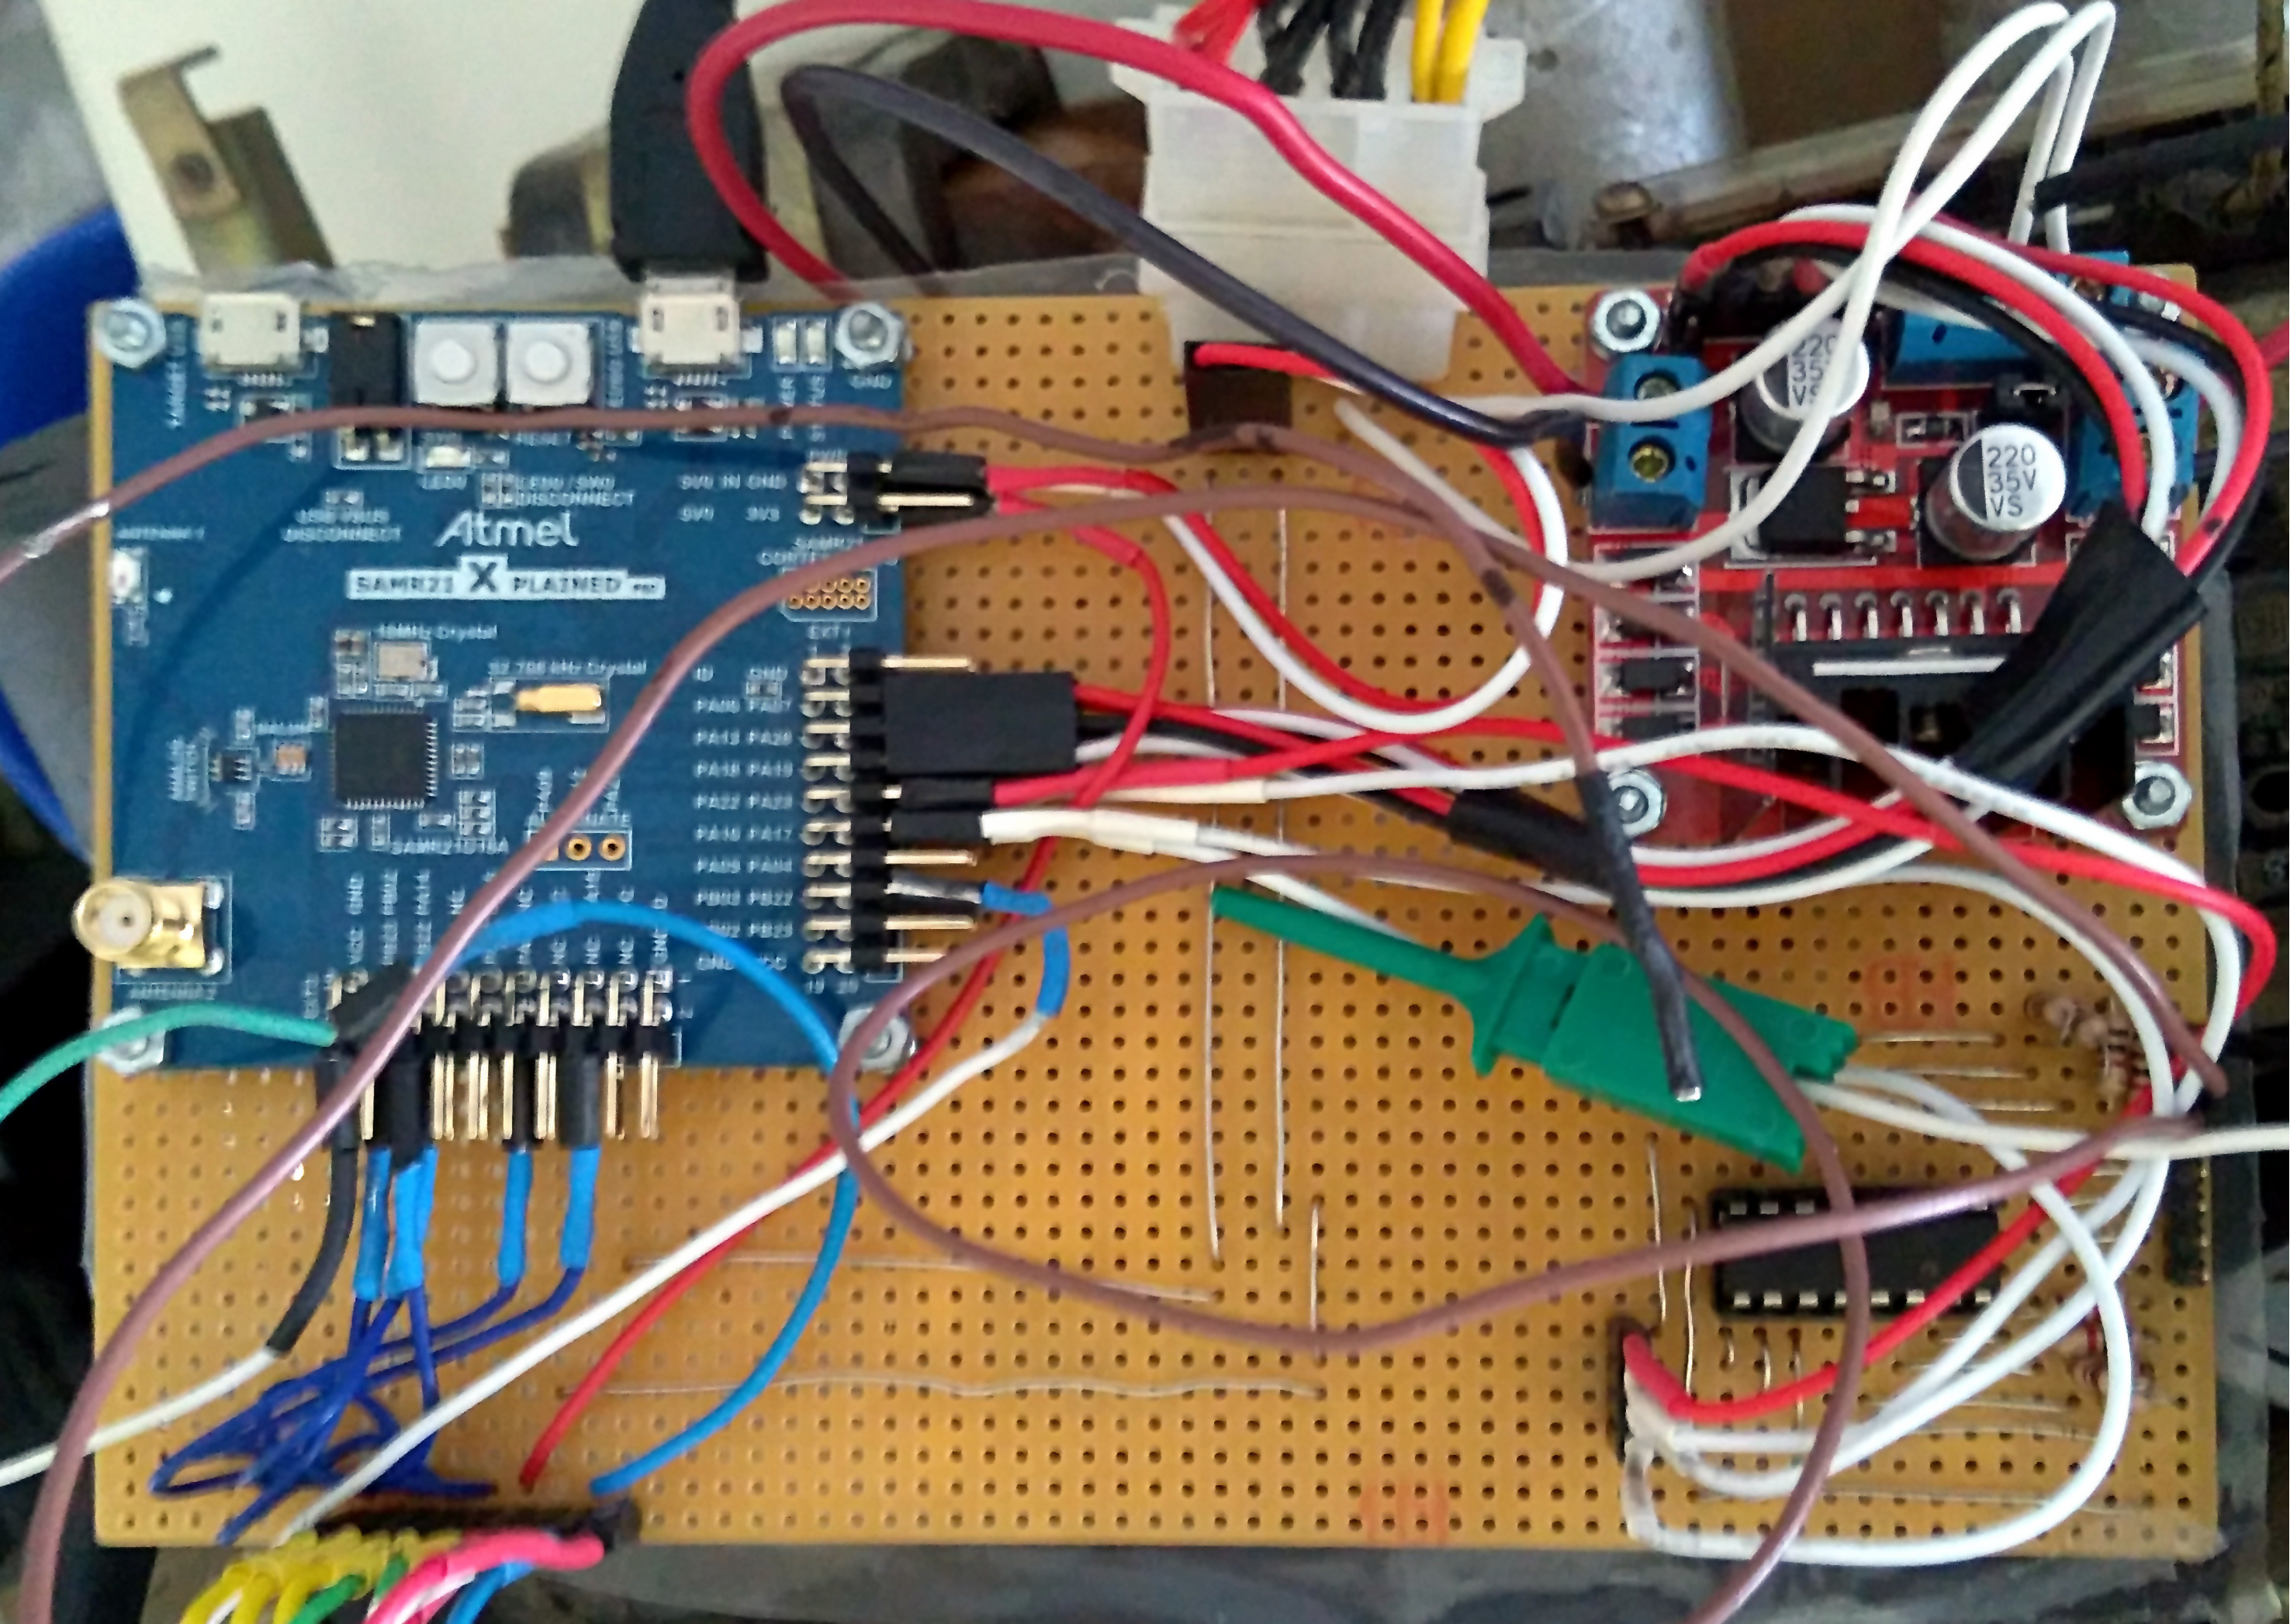
\includegraphics[scale=0.05]{Platine.jpg}
      \captionof{figure}{Mikrocontroller, Multiplexer und H-Br"ucke}
    \end{wrapfigure}
    In Ermangelung ausreichender I/O-Pins haben wir uns deshalb entschieden die Taster "uber den
    \textit{S74LS151}\footcite{S74LS151} zu verwalten. Der \textit{S74LS151} ist
    ein \( 8 bit \) Multiplexer und erm"oglicht es uns alle Taster mittels Polling abzufragen,
    allerdings kann immer nur ein Taster gleichzeitig mit einem Interrupt belegt werden.\\ Zur
    Beleuchtung der Bandlaufwerke haben wir RGB-LED-Streifen verbaut. Diese LED-Streifen sind
    kompatibel zu \textit{WS2811}\footcite{WS2811}, der jeweils eine LED steuern und bis zu 1024 mal in Reihe
    geschaltet werden kann um komplette Animationen darzustellen. Die existierenden Gl"uhlampen der
    Taster wollten wir ebenfalls durch LED's ersetzen die auf dem \textit{WS2811} basieren,
    allerdings gab es hier Lieferprobleme.\\
    \begin{wrapfigure}{r}{0.5\textwidth}
      \centering
      \label{figure:Bandlaufwerke}
      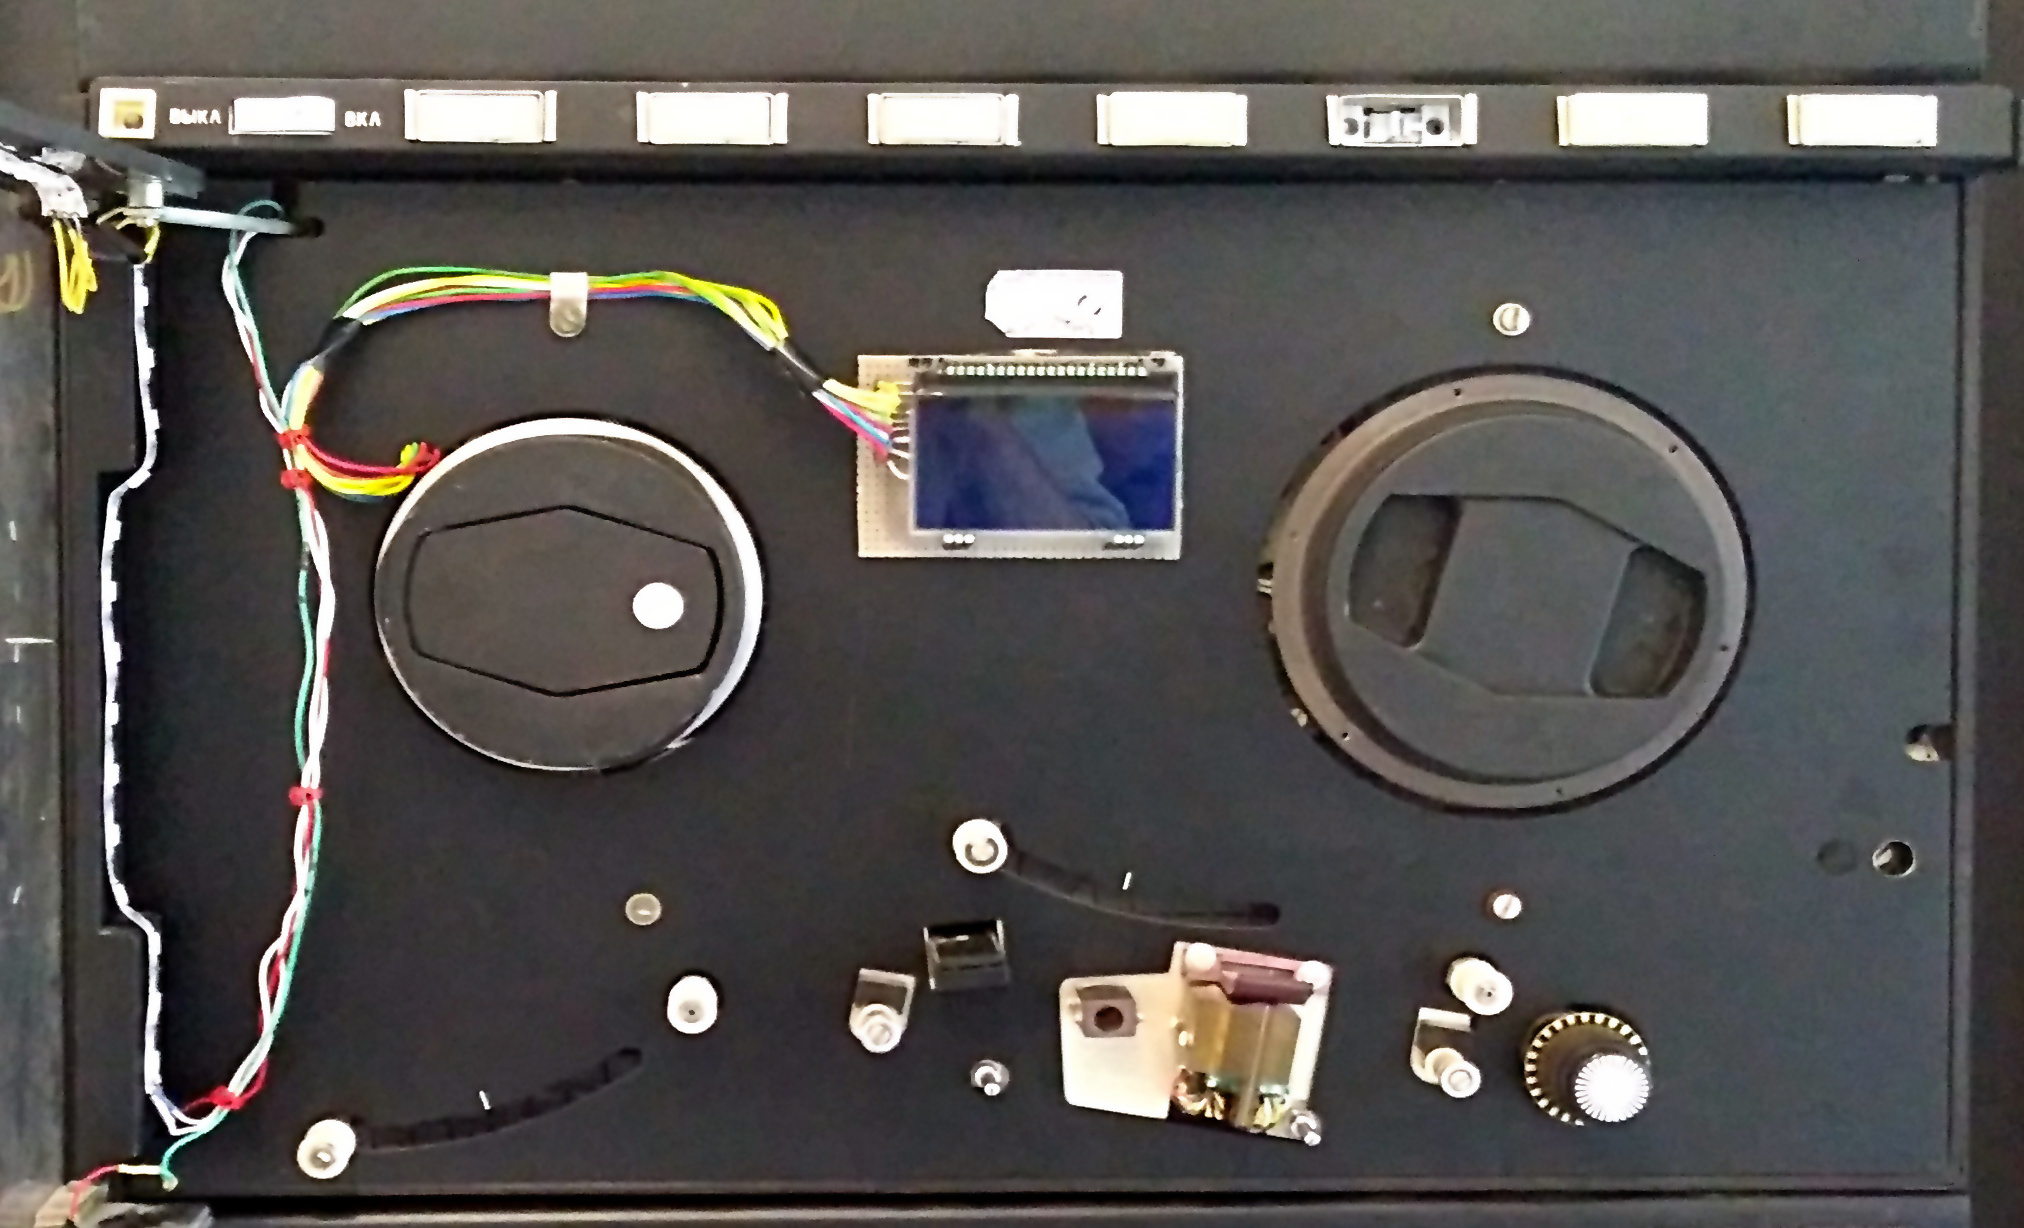
\includegraphics[scale=0.075]{Frontansicht.jpg}
      \captionof{figure}{Frontansicht der Bandlaufwerke}
    \end{wrapfigure}
    Zur Ansteuerung der Bandlaufwerkmotoren verwenden wir die doppel H-Br"ucke
    \textit{L298-H}\footcite{L298H}. Diese ben"otigt als einziges Modul eine 12V
    Versorgungsspannung.\\ F"ur zuk"unftige Men"uf"uhrung, Eingabe der
    Nicknames und weiteres visuelles Feedback haben wir ein 128x64 Pixel LCD
    des Typs \textit{DOGL128B-6}\footcite{DOGL128B} verbaut. Dieses Display ist ein Set aus
    Display und Controller und kann einfach "uber das SPI Protokoll verwendet
    werden. Um Kosten an der Hardware zu sparen haben wir uns dazu entschieden
    kein zugehöriges Backlight dazu zukaufen, sondern jeweils zwei
    \textit{WS2811} RGB-LEDs f"ur die Hintergrundbeleuchtung zu verwenden.\\
    Unsere verbaute Hardware braucht eine \( 3,3 V \), \( 5 V \) und \( 12 V \) Spannungsversorgung
    und anstatt ein neues Netzteil zu kaufen, haben wir ein ATX-Netzteil aus Restbest"anden f"ur beide
    Bandlaufwerke benutzt.

  \subsection{Treiber}
    \label{sec:hardware_driver}
    Nach der Entwicklung der Hardwareplattform haben wir f"ur jede Peripherie
    einen Teiber entwickelt, da diese noch nicht von RIOT selbst unterstützt
    wurden. Jeder Treiber ist angelehnt an die von RIOT angebotenen
    Beispieltreiber implementiert. Die Treiberimplementierung war für alle
    Peripheriegeräte außer dem \textit{WS2811} unkompliziert. Der
    \textit{WS2811} nutzt eine Schieberegisterarchitektur.  "Uber einen
    digitalen Eingang zum Empfang und einen digitalen Ausgang zum Senden an den
    nächsten \textit{WS2811} in Reihe werden je LED \( 24 bit\) an
    Farbinformationen "ubertragen.  Jeder \textit{WS2811} steuert eine LED und
    bis zu 1024 \textit{WS2811} können so miteinander verkettet werden, um ganze
    LED-Arrays zu steuern. Da der \textit{WS2811} nur ein OneWire-Protokoll und keine
    zusätzliche Taktung anbietet, benötigt er für die Unterscheidung zwischen 0
    und 1 in seinem Protokoll harte Timings. Für unser Projekt haben wir zwei
    verschiedene \textit{WS2811} kompatible LED-Sets gekauft. Das erste ist ein
    bereits montierter LED-Streifen, der mit unserem Treiber tadellos
    funktioniert und das zweite ist ein Set von separaten Chips und LEDs, die
    selbst zusammenzubauen sind. Das zweite Set weigerte sich, mit unserem
    Treiber zu arbeiten und nach mehrtägigem Debugging stellte sich heraus,
    dass der Controller eine gemeinsame Annode benötigt, aber die LEDs, die wir
    erhalten haben, boten eine gemeinsame Kathode.  Leider war der
    Internetversand, bei dem wir die LEDs gekauft haben, nicht in der Lage, die
    richtigen LEDs rechtzeitig zur Verfügung zu stellen, um das Projekt
    komplett abzuschließen.

\section{Retro11}
  \label{sec:retro11}
  \textit{Retro11} ist der Name der RIOT-Anwendung die auf dem \textit{SAMR21
  Xpro} l"auft. Die Anwendung besteht aus drei Teilen. Als erstes ist in
  \textit{Retro11} das Reaktionsspiel implementiert, das auch die Kontrolle
  "uber die gesamte Peripherie ben"otigt. Als zweites enth"alt jeder
  \textit{Retro11} Knoten einen COAP-Server der Anfragen vom
  \textit{Game-Master}-Knoten entgegennimmt. Als drittes und letztes l"auft auf
  einem Knoten zus"atzlich der \textit{Game-Master}-Knoten, der die ablaufenden
  Spiele koordiniert und die Ergebnisse an den RasperryPi von \textit{Team2}
  ver"offentlicht.

  \subsection{Anwendungsdesign}
    \label{sec:retro11_design}
    Als erstes initialisiert \textit{Retro11} die gesamte Peripherie und
    startet bis zu f"unf Threads, die "uber eine Message-Queue sowie eine
    geteilte Statusvariable kommunizieren.\\ Der erste Thread ist der
    \textit{MotorController}, der sich um die asynchrone Steurung der beiden
    Gleichstromotoren k"ummert. Dieser Thread akzeptiert Nachrichten, die die
    Geschwindigkeit und die Laufdauer der Motoren enth"alt. Dieser Thread ist
    essentiel f"ur das Reaktionsspiel, da die Motoren sonst nicht asynchron zur
    Benutzereingabe angehalten werden k"onnten.\\ Der zweite Thread ist der
    \textit{COAPServer}, der Anfragen des \textit{Game-Masters} erwartet und
    dann durch eine geteilte Status Variable die Game-Loop des
    Reaktionsspielthreads kontrolliert.\\ Der dritte Thread ist das
    Reaktionsspiel, das in der Endlosschleife GameLoop l"auft und durch die mit dem
    \textit{CoapServer} geteilte Statusvariable kontrolliert wird. Weiterhin
    kommunizert dieser Thread wie oben erw"ahnt mit dem
    \textit{MotorController} und bildet das Herzst"uck von \textit{Retro11}.\\
    Der vierte Thread stellt eine Diagnose-Shell "uber den USB-Anschluss des
    \textit{SAMR21 Xpro} bereit. In dieser Shell sind spezielle
    Hardware-Diagnose Befehle enthalten und au"serdem werden Debuginformation
    "uber den derzeitigen Programmverlauf ausgegeben.\\ Der f"unfte und letzte
    Thread ist nur auf einem der beiden Knoten vorhanden und stellt den
    \textit{Game-Master} zur Verf"ugung. Dieser kommuniziert mit den beiden
    \textit{CoapServern} und kontrolliert den gesamten Spielablauf zwischen den
    beiden Knoten. Der \textit{GameMaster} kommuniziert au"serdem mit dem
    RasperryPi von \textit{Team2} und ver"offentlich die Spielergebnisse.

  \subsection{Reaktionsspiel}
    \label{sec:retro11_game}
    F"ur dieses Spiele befinden sich zwei Spielende vor je einem Bandlaufwerk.
    Zuerst werden beide aufgefordert einen Nickname einzugeben, der dann an den
    \textit{GameMaster} geschickt wird. Sobald beide Spielenden ihren Namen
    eingegeben haben, sendet der \textit{GameMaster} den Start-Befehl und die
    Motoren beginnen sich zu drehen. Nach einer zuf"allig gew"ahlten Zeit
    h"oren beide Motoren auf zu drehen und die Spielenden m"ussen m"oglichst
    schnell den Best"atigen-Knopf dr"ucken. Die Zeit zwischen dem Anhalten
    der Motoren und dem Dr"ucken des Knopfes ist die Reaktionszeit und wird von
    beiden Knoten an den \textit{GameMaster} geschickt. Dieser entscheidet nun
    welcher der beiden Spielenden gewonnen hat und ver"offentlich das Ergebniss
    in der Highscore. Den Highscore k"onnen Sie in der Webapplikation von
    \textit{Team2} des diesj"ahrigen Softwareprojekts nachschlagen.

  \subsection{Netzwerkkommunikation}
    \label{sec:net}
    Die Kommunikation zwischen den Plattformen erfolgt über das RESTful
    Constrained Application Protocol, CoAP\footcite{COAP}, das Nachrichten über UDP und IPv6
    sendet, wie in Abbildung \ref{fig:seq_diagram} . Ein Mikrocontroller führt
    eine Client-Application aus, die das Spiel steuert. Die benötigten
    Informationen werden von einer Server-Anwendung bereitgestellt, die auf
    jedem Mikrocontroller ausgeführt wird. Abhängig vom Spielstatus fragt der
    Client die Ressource mit den erforderlichen Informationen beider Server mit
    einer Get-Methode ab, bis die Server die Informationen bereitstellen, um
    zur nächsten Stufe überzugehen.  Im ersten Zustand ruft der Client die
    Nicknamen der Spielenden ab, fordert dann das Reaktionsspiel auf, im
    zweiten Zustand zu starten, erh"alt im dritten Zustand die Reaktionszeit
    und fordert anschließend jede Maschine auf, anzuzeigen, ob der Spielende
    gewonnen oder verloren hat.  Zusätzlich verfügen beide Server über eine
    Ressource, die auf Wunsch von \textit{Team2} Highscore-Informationen im
    SenML-Format\footcite{SENML}
    bereitstellt.
    \begin{figure}[h]
      \centering
      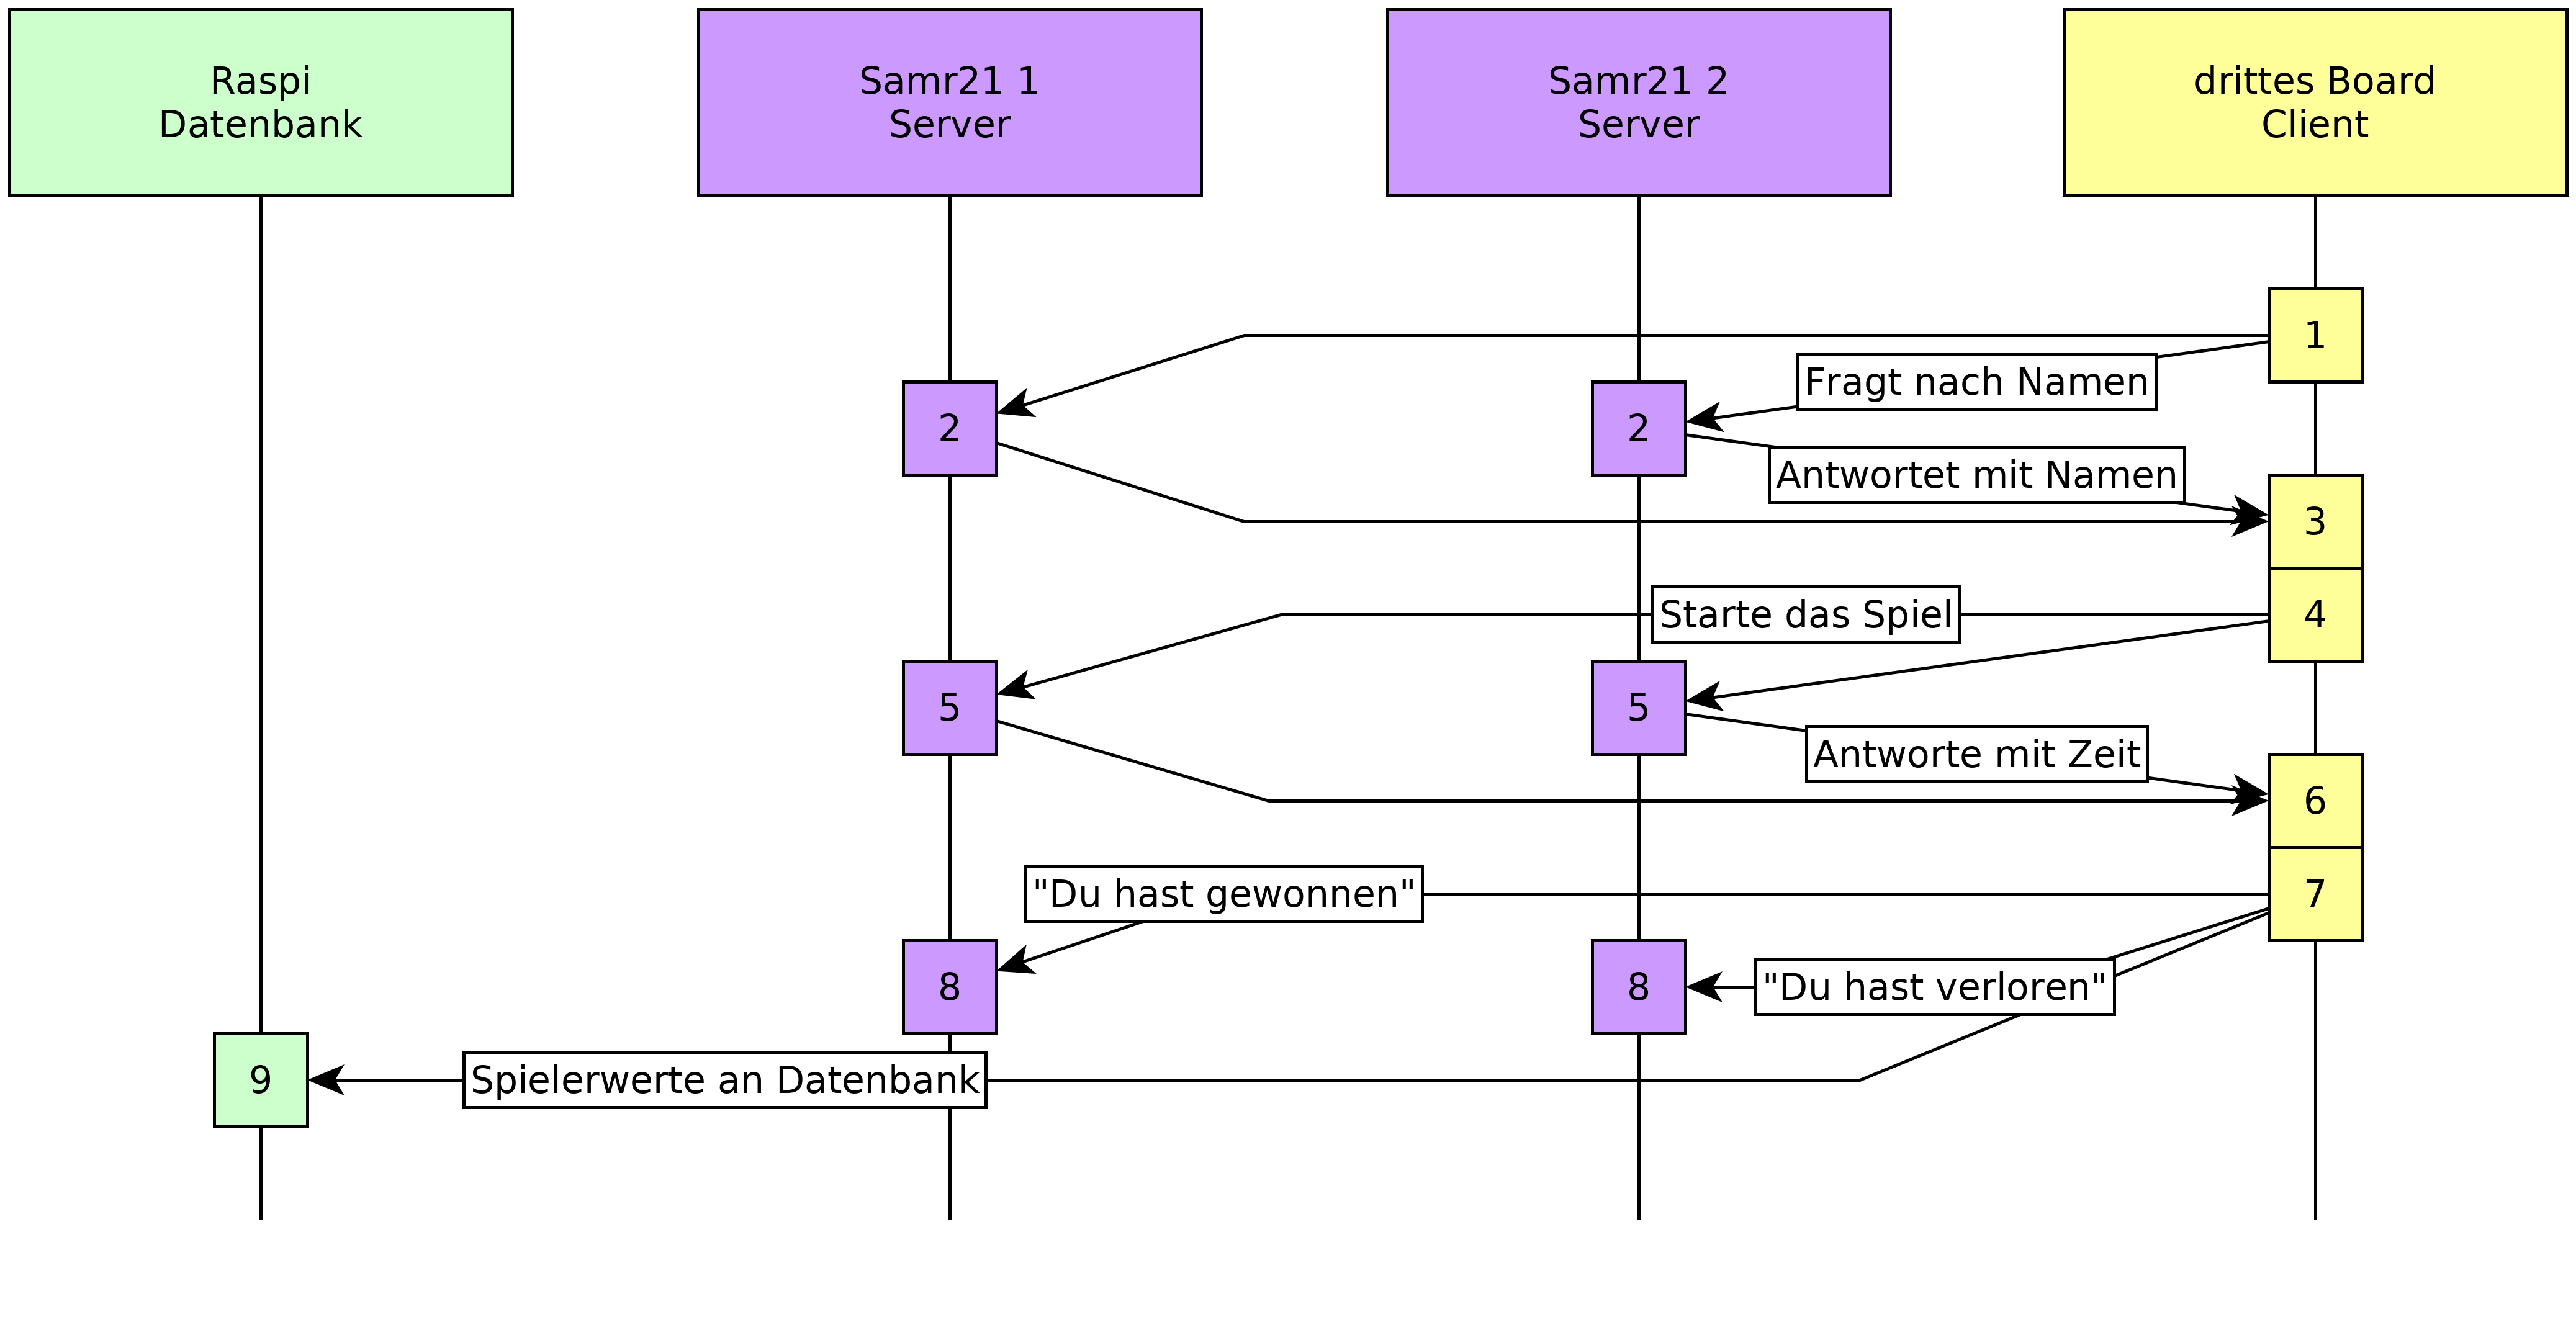
\includegraphics[scale=0.1]{team1_kommunikation.png}
      \caption{\label{fig:seq_diagram}Sequenzdiagramm der Anwendung}
    \end{figure}

\section{Stand der Umsetzung}
  \label{sec:status}
  \subsection{Probleme}
  In der aktuellen Implementierung bleiben noch ein paar Vorhaben unvollendet.
  Zum einen fehlen wie bereits erw"ahnt die passenden LEDs zu den
  \textit{WS2811} Controllern für die Taster. Weiterhin gibt es eine
  ungekl"arte Fehlerquelle im Zusammenhang mit einem der LCD. Hier scheint
  ein Wackelkontakt oder falsch eingestellter Kontrast zu einem unlesbaren
  Display zu f"uhren. Da das gleiche Programm auf dem anderen LCD zu einer
  Ausgabe f"uhrt erwarteten wir keinen Softwarebug. Das Ausmessen der
  Stromleitungen und das R"uckverfolgen der GPIO-Portleitungen hat allerdings
  keine Fehlerursache offenbart. Desweiteren existiert kein Boardlayout von dem
  Mainboard, welches die einzelnen Hardwarebausteine verbindet.\\ Die
  Netzwerkkommunikation ist derzeit unzuverla"ssig. Verlorene Pakete können in
  gewissen Situationen zu Deadlocks f"uhren.\\
  Zus"atzlich zu den offenen Problemen an unserem Projekt ist die Integration
  in das Softwareprojekt von \textit{Team2} ungen"ugend. Die Schnittstelle zur
  "Ubertragung der Highscoredaten wurde nur grob kommuniziert, nicht getestet
  und ist unseres Wissens nach nicht in der aktuellen Version von
  \textit{Team2} eingebunden.
  \subsection{R"uckblick auf Zeitplan}
  Der urspr"ungliche Zeitplan konnte aus folgenden Gr"unden nicht eingehalten werden.
  Die Entwicklung von Hardwarel"osungen und das Umsetzen dieser L"osungen haben
  ein Vielfaches der geplanten Zeit in Anspruch genommen. Zudem kostete das
  Debugging der \textit{WS2811} und der zugeh"origen LEDs unerwartet viel Zeit.
  Dies war besonders schwer einzusch"atzen, da die \textit{WS2811} kompatiblen
  LED-Streifen mit der gleichen Software funktionierten und so die Fehlersuche
  vielversprechend schien. Leider konnte dennoch der Fehler wie erw"ahnt nicht
  behoben werden. Weitere Ursache f"ur die Verz"ogerung waren Probleme mit der
  Netzwerkkommunikation und der langwierigen Integration der
  Netzwerkarchitektur in die "ubrige Projektstruktur, was letzendlich auch zu
  einer mangelhaften Schnittstellendefinition zwischen Applikation und
  Netzwerkarchitektur f"uhrte.\\ Als Ergebnis dieser Verz"ogerungen haben wir
  gewisse Vorhaben nicht umgesetzt, so haben wir zum Beispiel nicht nach
  passenden Magnetb"andern gesucht.\\ Das Implementieren des Spiels ging dann
  am Ende erwartungsgem"aß schnell und auch der Entwurf des Posters war
  entsprechend dem Zeitplan fr"uh beendet.\\ Eine Hauptursache f"ur das
  Nichteinhalten des Zeitplans waren fehlende Gespr"ache über den aktuellen
  Stand der Einzelaufgaben. So fehlte es der Gruppe an Wissen über den
  Fortschritt der Gruppenmitglieder und Probleme konnten nicht gemeinsam
  gel"ost werden.  Grund daf"ur sind aus unserer Sicht Erfahrungsmangel in
  der Projektarbeit und eine fehlende Gruppenstruktur.

\section{Weiterführende Arbeit}
  \label{sec:further}
  Zuerst gilt es die bis jetzt nicht gelieferten RGB-LED's wie in Abschnitt
  \ref{sec:hardware_additional} beschrieben in die Taster einzubauen. Bis jetzt
  werden die zu dr"uckenden Taster nicht visuell hervorgehoben, sodass f"ur
  Nutzer nicht offensichtlich ist welcher Taster welche Funktionsbelegung
  hat.\\ Zur weiteren Versch"onerung der Bandlaufwerke sollten die fehlenden
  Tasterfronten gedruckt werden. Ein druckfertiges 3D-Modell ist schon im
  Repository vorhanden. Im Zuge dessen sollten auch die Motoren gereinigt
  werden, da sie sich zur Zeit erst bei einer verh"altnism"a"sig hohen
  Anlaufspannung in Bewegung setzen. Dies w"urde Lautst"arkeentwicklung und
  Stromverbrauch optimieren.\\ Im Bezug auf \textit{Retro11} sollte als erstes
  ein Framework entwickelt werden in dem weitere Spiele implementiert werden
  k"onnen.  Eine M"oglichkeit besteht darin einen Lua-Interpreter in
  \textit{Retro11} einzubetten. interessierte Studierende sind dann in der Lage
  Spiele in einer Hochsprache gegen eine konsistente API zu entwickeln und
  m"ussen nicht notwendigerweise mit RIOT vertraut sein. Insbesondere f"ur
  Programmierneulinge bietet das einen niederschwelligen Einstieg in
  eingebettete Systeme.\\ Da regelm"a"sige manuelle Updates der vorhandenen
  Spiele auf der Plattform ein zeitintensives Unterfangen ist, sollte als
  n"achstes "uber eine Over-the-Air Updatefunktion f"ur die komplette
  Applikation oder zumindest f"ur die Spielebibliothek nachgedacht werden. F"ur
  RIOT selbst ist gerade ein OTA-Update in Entwicklung das nach Fertigstellung
  genutzt werden kann.\\\\

  \printbibliography

\end{document}
